\documentclass[10pt,letterpaper,oneside]{book}
\usepackage[spanish]{babel}
\usepackage[utf8]{inputenc}
\usepackage{enumitem}
\usepackage{color}
\usepackage{hyperref}
\usepackage{graphicx}

\newenvironment{myepigraph}
  {\par\hfill\itshape
   \begin{tabular}{@{}r@{\hspace{2em}}}} % 2em from the right margin
  {\end{tabular}\par\medskip}
\usepackage[left=2.2cm,right=2.2cm,top=2cm,bottom=2cm]{geometry}
\author{Z. López, M. Lara, E. Ocampo}
\title{Proyecto Educativo Semilla. Resumen}
\begin{document}
%MCEPASTEBIN%
\maketitle
\tableofcontents

\chapter{Introducción}

\begin{myepigraph}A fundamental concern for others\\
in our individual and community lives\\
would go a long way in making the world the better place\\
we so passionately dreamt of.
\vspace{0.1cm}\\
Nelson Mandela
\end{myepigraph}

\section{Presentación}

Somos Zitlali López, Manuel Lara y Eduardo Ocampo. Estamos convencidos de que podemos aportar de forma importante al desarrollo social en el sector educación, pues ahí convergen muchos de nuestros intereses, pasiones y habilidades. Identificamos en la educación básica un momento clave para el desarrollo ulterior de ciudadanos integrales en el cual podemos incursionar con ideas novedosas, profesionales y basadas en el más profundo deseo de mejorar la situación actual de la sociedad.

Planteamos un proyecto educativo que consiste de una Escuela y un Centro de Investigación Pedagógica (CIP) que funcionarán en la práctica como una misma entidad. Nuestro proyecto estará cimentado en cuatro ejes fundamentales: la {\bf felicidad} basada en la formación integral, vivir la {\bf democracia} participativa, la {\bf disciplina} no autoritaria, que emerge del trabajo naturalmente cuando éste nos motiva y, por último, promover y adoptar una actitud de {\bf exploración} hacia el conocimiento; esto último implica el reconocimiento del carácter dinámico y pragmático del mismo. Nuestro modelo pedagógico es Freinet y estará basado en actividades: buscamos un aprendizaje significativo a través del \emph{hacer}, pues estamos ciertos de que el conocimiento es relevante y pertinente en gran medida por su utilidad. El Centro de Investigación Pedagógica se encargará de generar propuestas educativas concretas (actividades, material didáctico, etc.) siempre congruentes con los ejes de la escuela, actuales, innovadoras y dirigidas a formar comunidad y fortalecer a las familias de sus integrantes. En la escuela se ejecutarán las actividades propuestas, se reportará su efectividad y se elaborarán sugerencias para la mejora de dichas propuestas.
\vspace{1cm}
\begin{myepigraph}No esperes a hacer de tu hijo un buen hombre,\\
hazlo un buen niño.
\vspace{0.1cm}\\
Proverbio
\end{myepigraph}

\section{El proyecto}

\subsection{Objetivos}
Son objetivos del proyecto:
\begin{enumerate}
\item Sembrar la idea de que la congruencia es un elemento necesario para la felicidad y la sostenibilidad de la raza humana.
\item Procurar y promover la felicidad de sus integrantes.
\item Proveer de todos los elementos para propiciar el correcto desarrollo emocional de los estudiantes.
\item Fomentar la actitud de exploración. En el caso de los estudiantes, esto significa que proveeremos de todas las herramientas que sean necesarias para que el estudiante se sienta motivado para conocer el mundo que le rodea desde distintas perspectivas. Para los profesores, esto significa una actitud de búsqueda constante de material para relacionar los elementos del temario con el contexto de sus estudiantes. Para los integrantes del CIP, la actualización permanente del temario, estar al tanto de avances en educación y la capacitación constante de los profesores.
\item Impulsar la disciplina en sus integrantes, entendida ésta como el conjunto de métodos que permitan al individuo concretar sus metas idealizadas de la forma más eficiente posible, o en defecto, a adaptarse para proponer nuevas metas que, bajo la perspectiva de la experiencia adquirida, sean factibles y compatibles con el espíritu original que motivó la empresa.
\item La creación de un ambiente democrático, donde todos participen en la construcción de un estado de bienestar general.
\item Buscar la retribución económica justa por las labores realizadas.
\end{enumerate}

\subsection{Centro de Investigación Pedagógica}
El Centro de Investigación Pedagógica (CIP) es una de las propuestas más inovadoras del proyecto, lo diferencian de prácticamente cualquier institución educativa a nivel básico. En el CIP se realizarán investigaciones en educación de calidad internacional y se socializarán los resultados que deriven de ellas a través de la página del proyecto, de publicaciones en revistas arbitradas del área, en congresos que organizará el mismo Centro y congresos externos internacionales y nacionales, así como en un Seminario Permanente del cual serán partícipes los miembros del CIP y los profesores de la Escuela. Realizará además Talleres y Cursos para Profesores interesados. Estamos conscientes de que educar con calidad requiere partir de la experiencia, lo que implica que el entorno dicta los métodos con los que se implementará el temario oficial. Lo anterior no sólo motivará el aprendizaje y favorecerá la trascendencia de los conocimientos adquiridos, sino que representa una herramienta para generar comunidad y fomentar la unión familiar al incentivar intereses comunes entre hijos y padres.\footnote{Las brechas generacionales se agrandan cuando no existen intereses en común y creemos que esto es un elemento importante en la desintegración de las familias.} Los integrantes del CIP deberán, de forma obligatoria, impartir talleres a los estudiantes de la Escuela para conocer de primera mano sus intereses y su situación emocional y académica.
\subsection{Seminario Permanente}
La conexión fundamental entre el CIP y la Escuela será el Seminario Permanente. Éste será un espacio en el cual se discutirán los métodos de enseñanza que se aplicarán en el salón de clases y aquellas experiencias que fueron positivas en la transmisión del conocimiento y/o en el cumplimiento de los objetivos del proyecto. Es en el Seminario donde el CIP dará a conocer las propuestas que resulten de su trabajo y el material generado y donde se capacitará a los profesores para que puedan desempeñarse de la mejor manera posible en sus aulas al implementarlos. También en este seminario los profesores darán testimonio del efecto que tienen las implementaciones previamente mencionadas en el salón de clases, se enlistarán las inquietudes que aparecieron frecuentemente por parte de los estudiantes y de los profesores para que el CIP pueda mejorar sus propuestas y/o la capacitación.

\subsection{La Escuela}
Iniciaremos la construcción de una escuela basada en el modelo activo y fundamentada en ideas de pedagogos que promueven los valores que nos identifican y que se plasman en la presentación. La escuela tendrá como principal activo  a sus profesores, quienes además formarán parte del Seminario Permanente de forma obligatoria, de tal forma que su trabajo será de tiempo completo.

Se le dará importancia primordial a la estabilidad emocional de los estudiantes, pues es parte del desarrollo integral y necesario para la el desarrollo de cualquier otra faceta del ser humano.

%escuela primaria se realizarán asambleas semanalmente en los salones y mensualmente se convocará a una asamblea de toda la escuela, como lo sugiere el método de Freinet. En el mismo tenor, se llevará un diario por grupo donde se relate lo acontecido en el grupo.

\chapter{Valores del Proyecto}

\begin{myepigraph}
Chi va piano, va sano e lontano.
\vspace{0.1cm}\\
Proverbio
\end{myepigraph}

\section*{Definiciones importantes}
\begin{itemize}

	\item {\bf Comunidad}	
La comunidad existe sólo cuando un conjunto de individuos, independientemente de su número, comparte problemas e intereses.
	
	\item {\bf Problema}
	Un problema es un hecho que usualmente representa alguna dificultad para un individuo o un grupo; esta dificultad donde se obliga a pensar en alternativas para superarla.
\end{itemize}

	\section{Democracia} 

		\subsection*{Definición}
La democracia es un proceso de gobierno que se puede desarrollar en cualquier tipo de comunidad (ver definición) para buscar el bien común. Se basa en la capacidad de sus miembros de escuchar y ser escuchados, así como de proponer y actuar -de forma prudente y responsable- en torno a los problemas e intereses que les conciernen.
	\vspace{-0.3cm}
		\subsection*{Elementos necesarios en una democracia}	
			\begin{itemize}
			\item La democracia se propone en una comunidad (revisar definición) cuyos individuos tienen interés por los problemas comunes y convencimiento de que se puede encontrar una solución.
			\item Se debe trabajar colectivamente en aproximarse a la solución de los problemas comunes.
			\item Deben encontrarse intereses comunes y establecerse, con base en ellos, objetivos comunes.
			\item Debe existir el interés por generar acuerdos que contemplen la visión de todos los integrantes de la comunidad. En caso de no existir, se debe fomentar el debate sano, entendiendo éste como uno donde se privilegie mejorar los argumentos de las posturas por encima de ``ganar'' el debate. También se deberá inculcar la disposición por ahondar en los intereses de los demás.
			\item Debe existir un ambiente de convivencia, donde se separen los ataques y elogios personales de la argumentación. Se deben poder identificar las falacias argumentativas y quitarles peso en la discusión.
			\item Un modo de proponer donde prevalezca, sobre la idea, los métodos. Sin duda es deseable que quien proponga coordine y asegure el desarrollo de sus propuestas.
			\item Disciplina. Sin esta característica, no se pueden concretar las ideas. Es fundamental. No debe tener la connotación de militarización, si no entenderse como un conjunto de hábitos que permiten a una persona realizar los proyectos que se proponga.
			\end{itemize}
	\vspace{-0.3cm}	
		\subsection*{Sobre el desarrollo de esta característica en los distintos sectores del proyecto (actividades, problemas y notas)}
			\begin{enumerate}[label=\Alph*]
			\item Estudiantes: 
		\begin{itemize}
		\item Asambleas. Se realizarán asambleas grupales y de toda la escuela. En las grupales, se resolverán problemas que surjan en el curso de las sesiones y que no puedan ser resueltos de forma inmediata, o bien que sean recurrentes. Cuando estos no puedan resolverse aún en la asamblea grupal o bien, cuando se trate de un asunto que involucre a gente fuera del grupo, se llevará el asunto a la asamblea de la escuela. En la asamblea general se tratarán entonces estos casos y también los maestros, la dirección y los miembros del CIP buscarán introducir dilemas para que sean resueltos por los estudiantes, como en qué invertir dinero en la escuela, o bien, cuestiones de interacción de la escuela con otras escuelas o comunidades.
		\item Consultas. Los estudiantes serán consultados para conocer su opinión respecto a ciertos aspectos referentes al crecimiento de la escuela; por supuesto, esta opinión será considerada con un fuerte peso para la toma de la decisión.
		\item Gestión de proyectos. Mensualmente, se les dará un prespuesto determinado a cada grupo para que definan algún proyecto y gasten dicho presupuesto.
		\item El problema de la educación como un problema de todos. Si un estudiante no está entendiendo algo, esto se entenderá como un problema para el salón en conjunto. La formas de abordarlos serán diversas, pero a manera de ejemplo se plantea generar una comisión para que estudiantes que entienden un tema puedan explicarlo a estudiantes que no lo entienden.
		\item La responsabilidad sobre el estado emocional de las personas tiene componentes colectivos. Cuando un estudiante tuviere un problema emocional, será deseable que los demás le expresen apoyo. Si hubiere un conflicto entre dos o más estudiantes, se tomará en tiempo en clase para intentar resolver el problema. Se promoverá que los compañeros no involucrados directamente en el problema propongan soluciones.
		\item Los niños ayudarán a limpiar lo que hayan ensuciado y a ordenar lo que hayan desordenado.
\end{itemize}					

			\item Profesores: 
			\begin{itemize}
			\item La forma de preparar las clases tendrá un componente democrático importante, pues en el seminario permanente se desarrollarán muchas ideas como resultado de compartir experiencias y del diálogo constructivo.
			\item Una vez consolidada la escuela, los socios fundadores promoverán que la nómina de profesores sea proporcional a las ganancias de la escuela.
			\item Buscaremos que la planta docente sea propositiva, de tal forma que se involucre naturalmente a los problemas del proyecto.
			\item Se impulsará que los profesores se involucren en actividades de socialización del conocimiento, sea mediante publicaciones o con actividades como parte de asociaciones civiles.
			\item Se promoverá una asamblea de la escuela donde se puedan resolver de forma pacífica y argumentada los problemas que surjan entre ellos.
			\item Participarán en el mantenimiento de las aulas en buen estado, esto es limpiando y ordenando.
\end{itemize}						
			
			\item Intendentes y Administrativos: 
\begin{itemize}
			\item Si es interés de ellos, podrán integrarse a cualquier actividad de la escuela. El CIP se encargará no sólo de gestionar la consolidación de sus propuestas, sino de promover que existan.
			\item Su labor será compartida por el resto de los miembros de la escuela.
\end{itemize}			
			
			\item Miembros del CIP: 
			\begin{itemize}
			\item Deberá, mediante el ejemplo, promover una forma de vida sana en comunidad.
			\item Impulsará un análisis sobre los argumentos, con miras a aclararlos y a objetivarlos. También promoverá en los miembros de Semilla el ser pertinente con los comentarios en asambleas.
			\item El CIP será el órgano que coordine las distintas actividades en donde se plantea un ambiente democrático.
			\item Buscará la forma de implementar una sana resolución de problemas.
\end{itemize}
			\end{enumerate}

	\section{Felicidad (a través de la formación integral)} 

		\subsection*{Algo como una definición de felicidad:}
		Una actitud hacia la vida que se caracteriza por la ecuanimidad y por la comprensión y la empatía hacia los problemas propios y ajenos.
		\subsection*{Profundizando sobre la definición:} 
		\begin{enumerate}[label=\alph*]
		\item Se nutre del reconocimiento de cada una de las facetas del ser (ej. nuestras formas de ser, nuestras emociones y nuestros patrones en distintos contextos: ser apegado, amoroso, enojón, etc.). Este reconocimiento se refleja en la manera en cómo uno responde ante las situaciones externas.
\item La felicidad lleva a buscar la solución de problemas desde la tolerancia (aceptando los desacuerdos y la confrontación, alcanzando la ecuanimidad)  y el trabajo constante. Para desarrollar la tolerancia parece ser muy importante el conocer distintas formas de vida y estar expuestos a ellas.
\item El estado de ánimo de una persona feliz se caracteriza por ser independiente de las condiciones externas inmediatas.
		\end{enumerate}

		\subsection*{Sobre el desarrollo de esta característica en los distintos sectores del proyecto (actividades, problemas y notas):}
			\begin{enumerate}[label=\Alph*]
			\item En general, para todos los integrantes:
			\begin{itemize}
			\item Se promoverá una forma de vida congruente y será un objetivo primordial de la escuela lograr consistencia entre los valores promovidos y la cotidianidad. Creemos que esto es clave para la felicidad.
			\item Se dignificará la labor de cada miembro de la comunidad, señalando lo imprescindible que son las labores de cada uno para el buen funcionamiento de la escuela.
			\item Se tomará en cuenta la voz de todos los miembros de Semilla para mejorar la situación de la escuela o para resolver problemas presentes.
			\item Las instalaciones serán bellas, provocando las sensaciones de bienestar que el contacto con la naturaleza suele generar.
			\end{itemize}
			\item Estudiantes: 
			\begin{itemize}
			\item Los niños deben disfrutar mucho el tiempo que están en la escuela.
			\item Una parte muy importante en la educación y a la que usualmente se le da poca importancia es el estado emocional de nuestros estudiantes. En Semilla los aspectos emocionales son de primera importancia e identificamos que sus soluciones deben de ser previas o simultaneas con el resto del aprendizaje. Resolver conflictos emocionales consideramos que forma parte fundamental de una vida feliz.

\end{itemize}			

			\item Profesores:
			\begin{itemize}
			 \item Queremos que nuestros profesores se den cuenta de lo importante que es su labor. Dignificando su labor seguramente fomentaremos que sean más felices, pues la realización personal está ligada de forma importante a la felicidad.
			 \item Se buscará que los profesores realicen su labor en un ambiente agradable.
			 \item Los directivos del proyecto apoyarán a los profesores en su desarrollo personal y profesional.
			 \item Nuestros profesores son de tiempo completo, buscamos darles un sueldo digno para dar a conocer lo importante que son para el proyecto.
\end{itemize}

			\item Miembros del CIP:
			\begin{itemize}
			\item De las ganas de vivir congruentemente con sus ideales es que el CIP debe laborar.
			\end{itemize}
			\end{enumerate}


	\section{Actitud de exploración} 

\subsection*{Sobre la definición:}	
		Explorar no es obtener respuestas, es una actitud y un conjunto de herramientas con las cuales se busca darle sentido al mundo para actuar en él, transformarlo y abordar los problemas que en él vayan surgiendo.

		\subsection*{Profundizando sobre la definición:}
		\begin{itemize} 
		\item El mundo hace referencia tanto al individuo como a su entorno y a las interacciones entre ambos. 
		\item En este sentido transformar el mundo incluye la transformación del mismo individuo, que usualmente sucede a través de la conformación de intereses.

\item En la exploración tienen lugar la observación, la curiosidad, la creatividad, el análisis (la comparación, la reflexión, la repetición) y la paciencia. Intuición, seguridad.
\item Explorar no es divagar, se realiza en conjunto con la construcción de un método para aumentar las probabilidades de éxito en la solución de los problemas, es decir, la exploración requiere de la disciplina.
\item Explorar no significa cambiar constantemente de intereses, requiere de un cierto compromiso para alcanzar metas.
\item Explorar no significa hacer lo que se desea, la apertura para explorar lo desconocido y lo impuesto (probablemente fuera de lo deseado por desconocido) lleva a la creación de nuevos intereses o a la reafirmación de los intereses existentes.

\end{itemize}

		\subsection*{Consideraciones sobre las formas de conocer:}
		El acercamiento hacia el conocimiento debe hacerse reconociendo que los seres humanos no enfrentamos algo nuevo con un completo desconocimiento sobre las cosas; los nuevos conceptos se construyen con base en lo que uno ya sabe. Podría suceder que las nuevas ideas no contengan significado para algún individuo, pero para dotarlas de significado el que instruye deberá partir de las estructuras previas en el individuo.
		
		\subsection*{Sobre el desarrollo de esta característica en los distintos sectores del proyecto (actividades, problemas y notas)}
		
			\begin{enumerate}[label=\Alph*]
			\item En general para todos los integrantes:
			\begin{itemize}
			\item Planear es algo deseable, sin embargo, no debe obstaculizar la realización de los planes. Frecuentemente se generan muchas ideas con buenas intenciones, pero no se llevan a cabo, no se concretan en actividades. Una de las razones de esto puede ser la creación constante de planes. Para acabar con esto, se propone tener una libreta de ideas, donde se pueden anotar todos los planes en cualquier momento. Sin embargo, cuando se está realizando una actividad, la exploración no debe interrumpirse por la planeación de otra cosa. Esto se parece un poco a la meditación, donde la mente debe enfocarse en una sola cosa durante un buen rato; mientras se explora, la mente puede vagar, pero debemos controlarla para llevar a buen término nuestra exploración. Las divagaciones pueden posponerse con ayuda de esta libreta.
			\item A pesar de que existen esquemas ya establecidos de trabajo, promoveremos que se utilice el sentido común para realizar las labores; no sin esto, dejar de cuestionar este sentido cuando sea pertinente, procurando su consistencia con la realidad.
			\item Consideramos que todos los integrantes del proyecto deben asumir una postura de exploración, generando así una capacidad de admiración por el mundo y sus procesos. También para ampliar nuestra capacidad de entendimiento y así, aumentar las probabilidades de ser feliz.	
			\end{itemize}
\pagebreak %AGUAS
			\item Estudiantes:
			\begin{itemize}
					\item Los por qués tan típicos en los niños de edades alrededor de 3 años, deben ser redirigidos para que el niño pueda formular posibles respuestas. No se debe desalentar el espíritu de búsqueda. Al darse cuenta un individuo de que es capaz de generar repsuestas, tendrá seguridad para ir planteando sus hipótesis y generar modelos del mundo.
					\item Se enseñarán métodos para llevar a buen término actividades por encima de conceptos. En este sentido, el esquema de competencias de la SEP se ajusta perfecto al proceder de Semilla y nos proporciona una plataforma sólida para educar.
					\item Los niños tienen intereses definidos ya cuando entran a la primaria y también en esta etapa se crean nuevos. Consideraremos los primeros como punto de partida para las actividades docentes, como propone Freinet y estamos conscientes del segundo punto, por lo que buscaremos {\bf generar} en los niños intereses consistentes con los valores del proyecto y el respeto a la naturaleza.
			\end{itemize}
			\item Profesores y miembros del CIP:
		\begin{itemize}
				\item Para educar creemos que se debe atender a la realidad. Decir que ésta se encuentra en constante evolución es afirmar lo obvio. Establecer un programa educativo que atienda la realidad requiere entonces de una evolución constante de los programas educativos, de las actividades en clase y del proceder en general del profesor. En este sentido, el profesor debe estar en constante exploración de formas, temas, chistes y demás componentes de una clase para educar contextualmente y pertinentemente.
				\item Se fomentará que los profesores sobrepasen esta exploración en el salón de clases y eventualmente socialicen sus hallazgos, sea en congresos, boletines y/o artículos.
		\end{itemize}
			\item Intendentes y Administrativos:
			\begin{itemize}
					\item Se promoverá que busquen constantemente mejores formas de realizar su labor.
					\item Se invitará a que participen en actividades fuera de sus labores, como son el seminario, congresos, etc. De tal forma que se fomentará la incursión de estos integrantes en programas que en otros sistemas educativos no forman parte de su quehacer.
					\item Se les invitará a actividades escolares de la escuela como son lecturas, salidas de campo, etc.
			\end{itemize}
\end{enumerate}
		
	\section{Disciplina}
		

		\subsection*{Sobre la definición:}
		Es conjunto de hábitos y habilidades que permiten a un individuo o colectivo alcanzar sus metas; o en su defecto, lograr adaptarlas para, con base en la experiencia adquirida, proponer nuevos objetivos concretos (que contenga el espíritu original) y buscar su realización.
		\subsection*{Profundizando en la definición:} 
		\begin{itemize}
		\item Una habilidad importantísima es generar el reconocimiento de las capacidades propias para lograr cierta(s) meta(s). Esto permitirá diseñar un plan de trabajo realista y por lo tanto, que pueda llevarse a buen término.
		\item Saber evaluar la pertinencia de la perseverancia para lograr la(s) meta(s) es indispensable para no caer en la terquedad.
		\item Cuando un individuo o colectivo se plantea sus propias metas es que la disciplina se vuelve fundamental en el desarrollo pleno del individuo o del colectivo.
		\item La disciplina es necesaria para lograr la libertad, pues nos permite \emph{hacer lo que queremos} en el sentido de que nos posibilita a 
		\end{itemize}


		\subsection*{Sobre el desarrollo de esta característica en los distintos sectores del proyecto (actividades, problemas y notas):}
			\begin{enumerate}[label=\Alph*]
			\item Para todos los integrantes:
			\begin{itemize}
					\item La disciplina militar (sobre todo en un salón) es además de anacrónica, indeseable para la formación de iniciativa y de creatividad. La falta de disciplina en virtud de la libertad creemos que lleva a la imposibilidad de la libertad misma, pues imposibilita al individuo la realización de sus proyectos y limita la autonomía fuertemente. Así es que la disciplina no es algo trivial ni binario; en Semilla se busca que la disciplina emerja del trabajo naturalmente.
			\end{itemize}
			\item Para los trabajadores de la escuela:
			\begin{itemize}
			\item Deben estar enamorados del proyecto Semilla. Debemos fomentar un ambiente laboral que motive a trabajar con gusto y con ánimo de mejora constante. Así es que se obtendrá la disciplina laboral que requiere el proyecto para funcionar.
			\end{itemize}
			\end{enumerate}


\chapter{Modelo Educativo}
\section{Las actividades}
En la escuela el trabajo se realizará a través de actividades clasificadas en las siguientes áreas: Madre Tierra, Comunicación, Artes y Oficios, Experimentación, Socioemocional, Deportes, cada una relacionada con las materias y el contenido que presenta el programa de la SEP y con el contenido que desarrolle el CIP. 

\vspace{0.5cm}
\begin{myepigraph}¿Por qué hay tanta gente sin tierra\\
habiendo tanta tierra sin gente?\vspace{0.1cm}\\
\\
Eduardo Galeano
\end{myepigraph}
\subsubsection{Madre Tierra}
El respeto por la Naturaleza, que es tan importante para sobrevivir como especie y para una vida congruente con los valores sociales actuales, se aprende en contacto con la Tierra. 

En ésta área se trabajarán con los niños actividades que promuevan una toma de consciencia sobre diferentes aspectos de la vida, como son el tener una alimentación saludable, la relación que tenemos con otros seres vivos, el impacto al ambiente generado a través de lo que consumimos de manera cotidiana, el sentido de formar comunidad para lograr un objetivo común. Para lograr lo anterior, se reconoce al Huerto Escolar como un lugar desde el cual se pueden introducir estos temas y entender la profunda relación que guardan unos con otros. Se estudiarán los contenidos de diferentes materias,  que comúnmente se presentan de manera aislada integrados en proyectos del huerto.  Todo esto, adecuándose de acuerdo a las necesidades diferentes de aprendizaje de los niños en cada grado escolar.
 
\vspace{0.5cm}
\begin{myepigraph} Todos los usos de la palabra para todos,\\
me parece un lema bueno y con agradable sonido democrático.\\
No para que todos sean artistas, sino para que nadie sea esclavo.\\
\vspace{0.1cm}\\
Gianni Rodari
\end{myepigraph}
\subsubsection{Comunicación}

El lenguaje está en la base del conocimiento (tanto al aprender como al compartir lo aprendido), de nuestras relaciones personales y de prácticamente cualquier aspecto de nuestra vida. 

En nuestra escuela la práctica comunicativa tendrá lugar a en el estudio de los contenidos de diferentes materias y en la expresión de los diferentes intereses (académicos y emocionales) que van surgiendo en el niño a lo largo de su educación básica.  Entre las actividades que se realizarán para lograr lo mencionado estarán el texto libre, diario escolar, la correspondencia, las conferencias, la lectura, cuenta cuentos, la declamación de poesía;  que ejercitan la sintaxis, la gramática, el vocabulario, la expresión oral y escrita, sin dejar de lado el uso de la tecnología como otra herramienta en esta práctica. 

\subsubsection{Artes y Oficios}

El arte y el oficio son un reflejo de las emociones, las costumbres, la historia, la diversidad cultural, que moldean al individuo. La complejidad en ésta área es el resultado de la confluencia de todo esto para lograr una expresión viva, tangible.

En esta área se trabajará integrando contenidos que harán posible el trabajo por proyectos y expresando libremente lo que el niño necesite. Para lograr esto, el niño llevará a cabo actividades en talleres creativos de pintura, escultura, fotografía, danza, carpintería, panadería, tejido, en los que conocerá el manejo de diferentes materiales y del cuerpo para lograr una obra plástica y escénica.  

\subsubsection{Experimentación}

Partimos del supuesto de que "la educación verdadera se logra mediante un principio general de experiencia por tanteo” (Frenet 1996: 34). El aprender a partir de la experiencia permite que el niño explore diferentes alternativas para acercarse a alguna posible respuesta a sus preguntas, a sus necesidades de conocer. 

En esta área el niño pondrá a prueba los supuestos con los que busca explicar las causas, procesos, consecuencias de algún fenómeno. Para ello los niños harán uso de la programación básica (robótica), las matemáticas, el método empírico y científico (cocina, huerto), de herramientas en el trabajo para alcanzar un objetivo individual y/o común. 

\subsubsection{Socioemocional}

La conformación de una personalidad democrática y la solución de conflictos constructivamente son primordiales para enfrentar retos en la actualidad. 

\vspace{0.5cm}
Las actividades que se realizarán están agrupadas en esta área son: 
\begin{itemize}
\item Críticas, felicitaciones y asambleas:

En los grupos los niños se felicitarán, criticarán y sugerirán formas de mejorar el ambiente del salón. Se realizarán asambleas semanales de toda la escuela que permitirán abordar problemas que identificarán y entre ellos buscarán una solución. 

\item Cocina y Limpieza:

El niño cocinará y limpiará su área y espacios de uso común, lo que ayudará en la formación de su independencia. 

\item Resolución de conflictos:
	
Se abordarán en el aula las situaciones de conflicto para reflexionar en conjunto sus causas y buscar de manera consensuada el construir un ambiente agradable de trabajo. Esto fomentará el autoconocimiento y la autodeterminación del niño.

\item Lectura de noticias:

Se abordará la lectura de noticias para fomentar en los niños la compasión y la comprensión de su estar en un tiempo y en un espacio determinado. Esto aportará elementos importantes para el análisis crítico de la realidad.

\item Tutorías:

Este es un momento en donde el niño entra en contacto directo con personas del ámbito artístico, humanístico, científico, tecnológico y de oficio, para que empiece a explorar y conocer qué es lo que actualmente se hace en distintas áreas del conocimiento y del campo laboral.

\item Ejercer un presupuesto:

A distintos grupos de nuestra escuela se les asignará un presupuesto para realizar alguna iniciativa colectiva. Con asesoría, los estudiantes deberán determinar cómo ejercerlo. El proyecto comprenderá desde la planeación hasta la realización.

\end{itemize}

\subsection{Nuestro Maestros:}

Los maestros son una parte fundamental del proyecto Semilla. Para lograr los objetivos planteados es necesario que identifiquen que la escuela, es un lugar en constante cambio, que debido a esto representa una oportunidad de transformación para ser una mejor persona. 

Hemos reflexionado que hay algunos aspectos que pueden llevar a que un maestro mejore su práctica día a día. Dentro de estos aspectos está la actitud que tiene consigo mismo y por otro lado la actitud que muestra en el acto educativo, aquella que se lleva a cabo en la escuela en la interacción cotidiana con sus estudiantes.

Queremos que nuestro maestro persiga ser congruente, honesto, explorador, comprometido, empático, auténtico, ecuánime y positivo. Además deseamos que el maestro en su práctica educativa reconozca que: 
\begin{enumerate}
\item ``Los niños quieren saber, quieren comprender, quieren actuar si nosotros les impedimos esto imponiéndoles cosas que no les interesan, se cerrarán cada vez más a nuestras enseñanzas y buscarán por otros caminos, otra forma de cultura.''
\item ``Concedemos mayor importancia a la adquisición básica de los conocimientos elementales, a las observaciones y a las experiencias que permiten la profundización de todos los problemas.''
\end{enumerate}

Freinet (2009). Consejos a los maestros jóvenes. 
Josep Colome (Trad.) p. 117-118. Obra original publicada en 1968.

\chapter{Socialización}

El proyecto tiene como objetivo formar una comunidad sólida que sea capaz de transformarse positivamente hacia las formas de pensar el mundo y de actuar en él que la misma comunidad determine como valiosas y/o necesarias, esto tomando en cuenta a la sociedad en general y la complejidad que le da vida. En otras palabras, pretendemos que el proyecto en su conjunto y a conciencia vaya más allá de la formación de niños, que rebase el ámbito escolar tradicional y que permee a padres, maestros, investigadores, administrativos y trabajadores, de modo que todos ellos se entiendan como una comunidad desde la cual busquen comprender la realidad que habitan, puedan tomar una postura ante ella y, más aún, que aspiren a transformarla crítica y colectivamente. 

Aunado a lo anterior, el proyecto tiene la intención de entablar relaciones, por medio del CIP, con grupos y sectores educativos que estén determinados a proponer y crear una educación distinta. La idea de ello es colocarse en una realidad social que va más allá del ámbito comunitario local para, con una mirada mucho más amplia, poder entender el papel y la dirección de los distintos esfuerzos educativos. En última instancia esto nos permitirá generar redes que le den solidez tanto a nuestro proyecto como a otros que, aún insertados en otras realidades locales, tengan como motor ideales e intenciones similares. En este sentido, pensamos que un cambio social es producto de la organización de los diversos esfuerzos locales por medio de redes robustas en las que puedan resonar las distintas voces y acciones que las conforman.
 
Es así que el CIP, más allá de organizar y darle consistencia a las propuestas en el ámbito escolar, se encargará de darle un sustento social al proyecto a través de:

\begin{enumerate}

\item La socialización de las experiencias escolares a través de diversos medios de acceso libre.
\item La generación de espacios en los que se lleve a cabo una discusión continua sobre el estado presente de la educación, los problemas que la aquejan y las diversas formas de abordarlos en la práctica, tanto en la escuela pública como en otros ámbitos educativos. Entre esos espacios, deseamos encaminar buena parte de nuestros esfuerzos a la organización de congresos y la creación de una revista.
\item La capacitación de maestros basada en: la práctica y el conocimiento desarrollados en la escuela, así como en las conclusiones sobre las necesidades sociales que se deriven de los espacios descritos en el punto anterior. Tal capacitación buscará entender la diversidad de contextos escolares, pero también buscará derribar los mitos generados en torno a las posibilidades de la escuela pública, dándole una importancia primordial a la capacitación de los maestros de esta última.
\item La consolidación de lazos con escuelas, centros de investigación educativa, propuestas educativas no escolarizadas y educadores independientes para generar las redes mencionadas.


\end{enumerate}

Para nosotros el aspecto social del proyecto no es una cosa accesoria que se incluye sólo como parte del discurso en boga, sino que es el corazón mismo del proyecto. Hemos decidido abordar la educación primaria porque vemos en ella los cimientos desde los cuales se puede modificar la dirección de una sociedad que entendemos como profundamente viciada. Queremos abandonar el aspecto meramente sonoro de palabras como democracia y felicidad, para aproximarnos a ellas seriamente y a profundidad, para investigarlas y vivirlas entendiéndolas como procesos que se deben cultivar y promover a lo largo de la vida, no como nociones que se decretan. Vemos en la escuela la posibilidad de construir una realidad social distinta a la dominante en la que, entre muchas otras cosas, se dignifique el trabajo, en la que se evite construir elites que pretendan imponerse y en la que quepan muchos mundos capaces de construirse en conjunto. Y creemos también que estas nociones se pueden contagiar mucho más allá de la escuela


\chapter{Plan de Negocios}

\section{Planeación Estratégica}
\subsection*{Misión}

Conformar una comunidad educativa que rebase el inmueble de la escuela y que logre penetrar las esferas de la cotidianidad en sus integrantes y en la comunidad donde está insertada, impulsando una forma de convivencia distinta, congruente con una forma de vida sostenible. La conformación de un espacio educativo y democrático, donde prevalezca una actitud de exploración ante la vida, donde se considere la felicidad como un valor supremo y se entienda la libertad como resultado de la congruencia entre lo que uno quiere y la forma en que se aproxima a ello. 
\subsection*{Visión}
Buscamos ofrecer educación de calidad, contar con miembros comprometidos con los estudiantes y con el país. Contamos con un equipo de científicos y pedagogos para diseñar estrategias educativas novedosas, profesionales y basadas en el más profundo deseo de mejorar la situación actual de la sociedad. Desde antes de iniciar operaciones, capacitaremos a nuestros profesores en ciencia, artes y el método Freinet. La capacitación docente será permanente desde entonces. Al año de conformación, se realizará el Primer Congreso Anual de Educación por una mejor Sociedad. Ahí se establecerán relaciones que ampliarán el espectro de posibilidades en el aula en nuestra escuela. En 1 año se realizarán las primeras publicaciones en el área de pedagogía. En 4 años contaremos con una matrícula de 20 estudiantes con 6 grupos de primaria. En 5 años seremos una de las mejores opciones educativas del estado para el sector progresista, con un método pedagógico propio, profesores de nivel, publicaciones en revistas arbitradas y se apoyarán proyectos sociales locales con recursos de la escuela.

\section{Descripción del Negocio}

Semilla es una escuela privada activa, así como talleres vespertinos donde el aprendizaje se centra en el estudiante. Es él quien debe tener la mayor participación en las clases, se busca que sea propositivo, que sepa comunicarse y que posea habilidades para llevar a buen término sus ideas. El proceder se basa en el desarrollo de actividades y no en la exposición tradicional donde el maestro dice y el alumno apunta e intenta memorizar. En Semilla, el estudiante \emph{hace} y es en la creación que surgen inquietudes y dudas, las cuales el profesor orienta para generar \emph{descubrimientos}. De la misma forma es que los aspectos emocionales serán tratados en Semilla, surgen en el quehacer cotidiano y el profesor, con ayuda de un equipo con fundamentación psicológica, dirige para que se lleven a buen término, buscando que el estudiante descubra sus emociones, las de los demás y encuentre métodos para empatizar y darse a respetar. El método pedagógico del que se parte en la primaria es el \emph{método Freinet}, puesto que otorga una plataforma probada en México y otras partes del mundo compatible con los principios expuestos previamente y detallados en la sección de \emph{Valores}. Bien hay gente que resume este método en \emph{darle la palabra al niño}.

\section{Análisis del Mercado}

Entendemos por competencia a escuelas primarias no religiosas, con un modelo pedagógico bien estructurado, bilingües y dirigidas el sector C, C+ y A. Nuestro mercado está conformado por padres de familia de estos sectores económicos, profesionistas y preocupados por el tipo de educación que reciben sus hijos, por encima del prestigio, de la apariencia. Un sector secundario está constituido por padres que no necesariamente sepan discernir cuál es la mejor opción para sus hijos, pero les atraigan los valores del proyecto y el método de actividades que se utiliza; este último sector resulta interesante en Tequisquiapan, donde gente de municipios aledaños puede desplazarse para darle a sus hijos una mejor opción educativa.

\subsection{Población de Tequisquiapan}





\subsection{Competencia}

La siguiente información obtenida desde la red \cite{mejoresescuelas}, mystery consumer y alianzas estratégicas.

\subsubsection*{Tequisquiapan}
\begin{center}
\begin{tabular}{|c|c|}
\hline 
{\bf Nombre} & Colegio Tahuilco \\ 
\hline 
{\bf Lema} & Lugar de luz, donde se disfruta el conocimiento. \\ 
\hline 
{\bf Precio} & • \\ 
\hline 
{\bf Ventaja competitiva} & Modelo Freinet y Pierre Faure, Instalaciones Bonitas \\ 
\hline 
{\bf Calidad} & • \\ 
\hline
{\bf Percepción} & • \\ 
\hline 
{\bf Ubicación} & Venustiano Carranza \\ 
\hline 
\end{tabular} 
\end{center}

\begin{center}
\begin{tabular}{|c|c|}
\hline 
{\bf Nombre} & Colegio Victoria \\ 
\hline 
{\bf Lema} & Instituto Bilingüe Victoria, A.C. \\ 
\hline 
{\bf Inscripción} &  \\ 
\hline 
{\bf Colegiatura} & 7,000 \\ 
\hline
{\bf Ventaja competitiva} & Bilingüe. Sistema Británico. Política Contra Acoso Escolar. \\ 
\hline 
{\bf Calidad} & NA \\ 
\hline 
{\bf Percepción} & 10 \\ 
\hline 
\end{tabular} 
\end{center}

\begin{center}
\begin{tabular}{|c|c|}
\hline 
{\bf Nombre} & Colegio Real de Querenda \\ 
\hline 
{\bf Lema} & Veni Vidi Vici \\ 
\hline 
{\bf Inscripción} & 5,520 \\ 
\hline 
{\bf Colegiatura} & 3,250 (10 meses) \\
\hline
{\bf Ventaja competitiva} & Bilingüe. Sistema UNO. De boca en boca se ha hecho famosa. \\ 
\hline 
{\bf Calidad} & NA \\ 
\hline 
{\bf Percepción} & 9 \\ 
\hline 
\end{tabular} 
\end{center}

\begin{center}
\begin{tabular}{|c|c|}
\hline 
{\bf Nombre} & Colegio Motolinía Tequisquiapan \\ 
\hline 
{\bf Lema} & Creatividad, Respeto, Felicidad, Conocimiento \\ 
\hline 
{\bf Inscripción} & 4,240 \\ 
\hline 
{\bf Colegiatura} & 1,800 \\
\hline
{\bf Material} & 750 \\
\hline
{\bf Tiendita AMCO} & 250 \\
\hline
{\bf Libros AMCO} & 3,940 \\
\hline
{\bf Ventaja competitiva} & Bilingüe. Sistema AMCO.\\ 
\hline 
{\bf Calidad} & NA \\ 
\hline 
{\bf Percepción} & 9 \\ 
\hline 
\end{tabular} 
\end{center}

\begin{figure}[h]
\centering
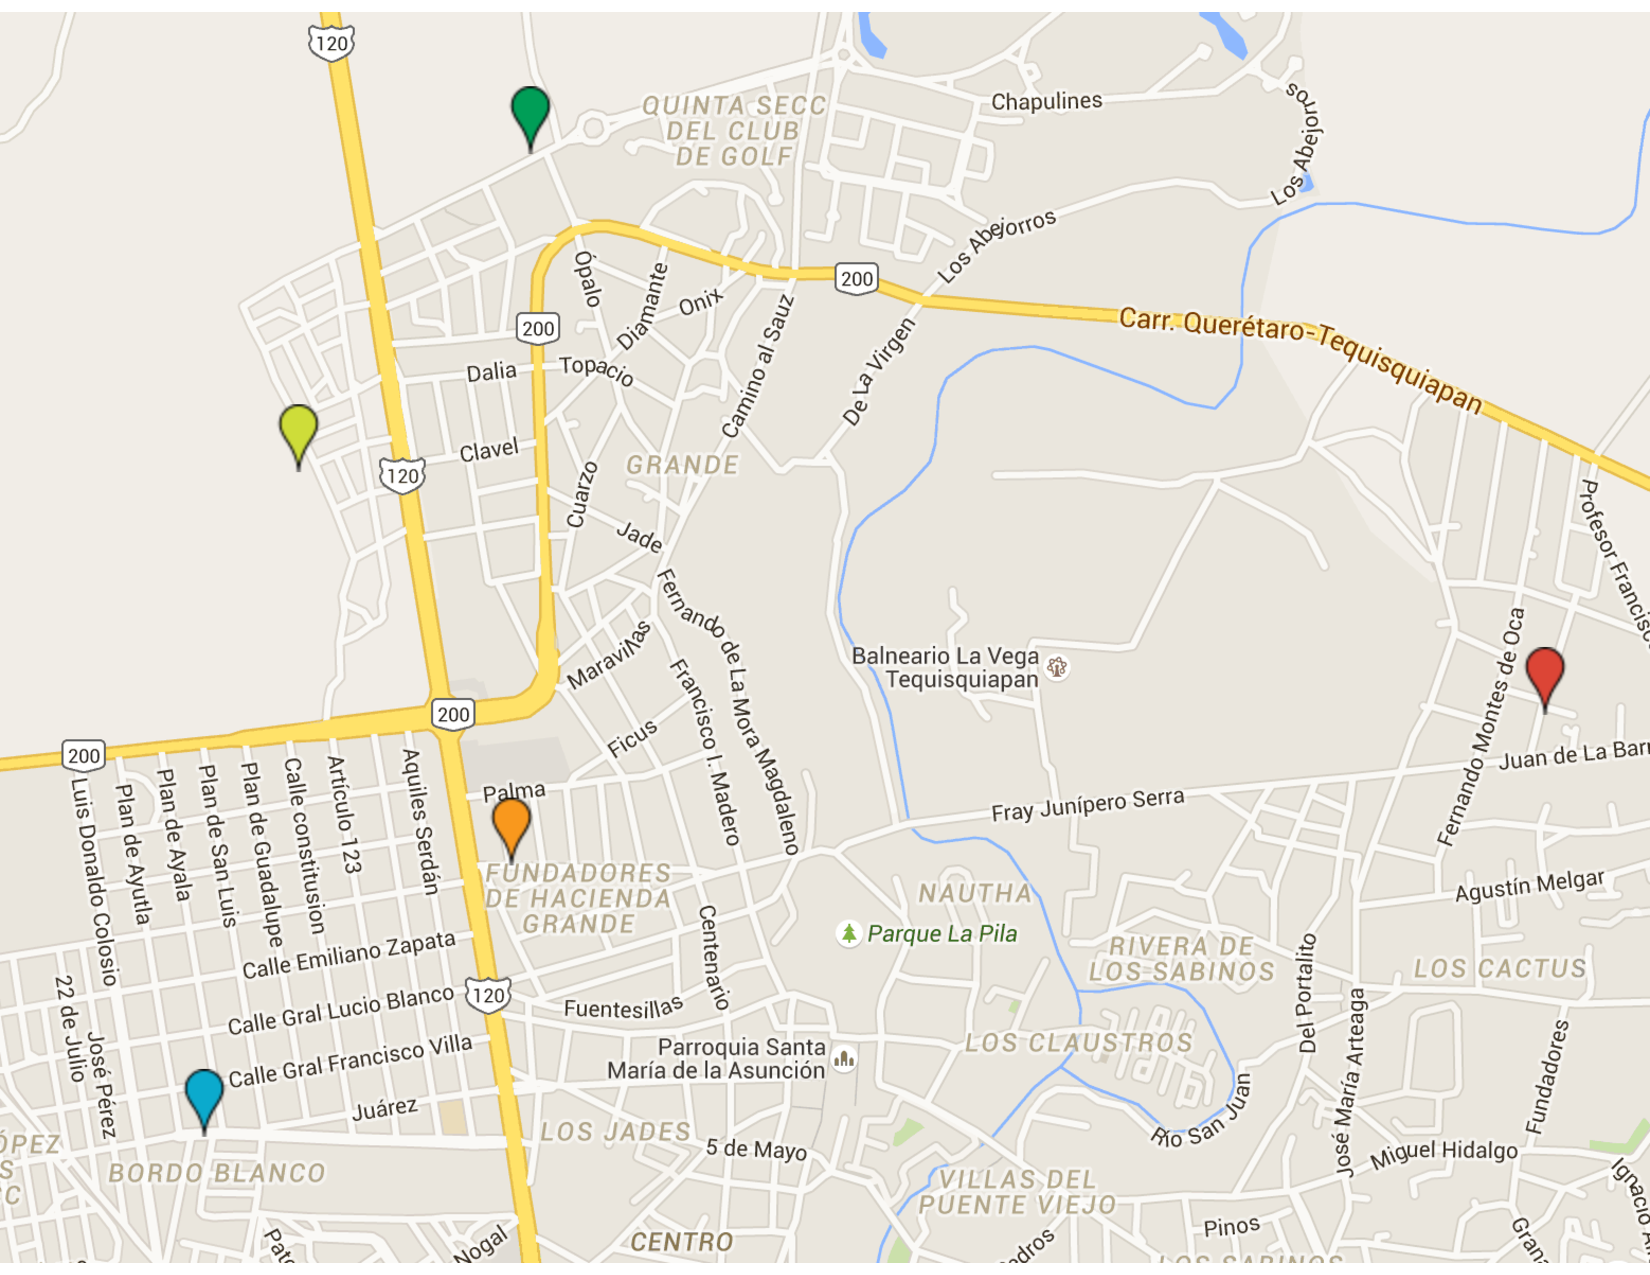
\includegraphics[scale=0.6]{mapatequis.pdf}
\caption{Ubicación de las escuelas que representan competencia en la cabecera municipal. Al norte, en verde oscuro el Motolinía, al este en rojo, el Colegio Victoria, al suroeste en azul el Tlahuilco y en fundadores hacienda grande, cerca de la carretera 120 el Querenda.}
\end{figure}

\section{Producto, Precio, Plaza y Promoción}

\subsection{Producto}
Servicio educativo a nivel primaria de calidad con un centro de investigación pedagógica, profesores de tiempo completo y capacitación docente permanente. También se ofrecerán talleres vespertinos con costo extra y capacitación a profesores externos; con costo para profesores de instituciones particulares y gratuitos para profesores de escuelas públicas. 


\subsection{Precio}
Se propone una colegiatura mensual de \$3,300.00, para primaria. Los talleres individuales costarán \$900.00-\$1,000 (más materiales) y los grupales \$330-\$600. 

\subsection{Plaza}

El terreno se encuentra en ``La Lagunita'', localidad de 52 habitantes por lo que puede considerarse rural. Se ubica a  1900m sobre el nivel del mar y en la salida a Ezequiel Montes. Cerca de la carretera y con una posibilidad grande de embellecimiento, el camino es de Tierra y hay casas relativamente bonitas. Planeamos sembrar plantas y árboles por la zona para mejorar su atractivo. Puesto que existen también clientes de otros municipios, este lugar es atractivo porque no necesitan cruzar la ciudad.

\subsection{Promoción}
Se realizará una estrategia de marketing que contemple redes sociales como el principal medio. Se realizarán alianzas con jardines de niños que no tengan primaria y con universidades para becar a su hijos de profesores e investigadores. Los congresos representarán una buena forma de publicidad, así como mesas redondas sobre el futuro de la educación en México con invitados de nivel.


\chapter{Modelo de negocio}

\section{Introducción}
A pesar de que Semilla será una institución privada, financiada por el cobro de colegiaturas, su finalidad última no es lucrativa, es social. En el apartado de ``Socialización'' se profundiza en esto.  Considerando lo anterior, resulta sumamente importante el diseño de un modelo de negocios finamente detallado, consistente y resiliente, pues el éxito del impacto social que nos impulsa depende directamente de la viabilidad y estabilidad financiera del proyecto.

\section{Sobre el trabajo en Semilla}
Una de las finalidades sociales del proyecto es la generación de empleos. Aunque el salario no es determinante en la dignificación de la persona, creemos que es un primer paso y que es muy importante en la sociedad contemporánea. Por un lado representa un avance en términos de equidad social, por otro le permite a nuestros trabajadores comprometerse con su labor sin sacrificar otros aspectos de su vida, brindándoles tranquilidad. Queremos ofrecer también las prestaciones de ley a nuestros trabajadores y, por encima de todo, un ambiente retador donde puedan crecer profesional y personalmente.

En estos tiempos, el reconocimiento social a la labor docente frecuentemente no corresponde a la importancia que ésta tiene en la sociedad. en Semilla buscamos cambiar este paradigma, partimos de que la docencia es una de las actividades más importantes en el quehacer humano y pugnaremos por honrarlo y promover que sea honrado.

\section{Sobre las Colegiaturas y las Becas}

Las colegiaturas estarán subsidiadas por los talleres vespertinos. Las colegiaturas se establecerán bajo el criterio de cobrar lo mínimo posible de colegiaturas y de forma que permitan:
\begin{enumerate}
\item cubrir los gastos corrientes de nómina y materiales;
\item poder pagar el mantenimiento de las instalaciones y los servicios públicos;
\item poder solventar la renta del lugar, o bien, amortizar las deudas de préstamos;
\item becar prácticamente al 10\% de la población estudiantil (2 de cada 20 aproximadamente) en comida, colegiatura, uniforme y útiles escolares;
\item financiar el Seminario de Capacitación Permanente y ciertas actividades enfocadas a mejorar la calidad docente;
\item rentar, poder financiar en 5 años el cambio a una localidad propia, más adecuada, con construcción natural, mayor espacio de recreación y más espacios con más posibilidades de actividades;
\item cuando se deje de pagar renta, o bien, préstamos, el excedente mensual se repartirá en su mayoría entre los integrantes de la escuela, se aumentará el número de becas sin aumentar en número de estudiantes por salón y se apoyarán proyectos culturales, sociales y académicos regionales.
\end{enumerate}


\section{Factibilidad del Modelo de Negocios: Ejercicio Anual Financiero Primaria}

Para una referencia completa, con todos los gastos desglosados y contemplados, revise el {\bf Anexo: Presupuesto}. Operando la escuela al 100\% de su capacidad, se tendrá la siguiente nómina:

\begin{center}
\begin{tabular}{|c|c|c|}
\hline 
{\bf Puesto} & {\bf Cantidad} & {\bf Salario Neto} \\ 
\hline 
Profesor frente a grupo & 6 & 18,000 \\ 
\hline 
Secretaría & 1 & 10,000 \\ 
\hline 
Velador & 1 & 10,000 \\ 
\hline 
Intendencia & 1 & 10,000 \\ 
\hline 
P. Educación Física & 1 & 10,000 \\ 
\hline 
P. Artes & 1 & 10,000 \\ 
\hline 
Contador & 1 & 1,000 \\ 
\hline 
Dirección & 1 & 20,000 \\ 
\hline 
Miembros CIP & 4 & 18,000 \\ 
\hline 
\end{tabular} 
\end{center}
y, entre otros, los siguientes costos importantes:

\begin{center}
\begin{tabular}{|c|c|c|}
\hline 
{\bf Concepto} & {\bf Costo}  \\ 
\hline 
Renta & 35,000 \\ 
\hline 
Gastos de Operación & 71,000 \\ 
\hline 
Renta & 35,000 \\ 
\hline 
Pago Préstamos (sólo cuando en opción de compra) & 70,000 \\ 
\hline 
\end{tabular} 
\end{center}
\vspace{0.3cm}
Nuevamente recordamos que en el {\bf Anexo: Presupuesto} está la información detallada, aquí sólo se presentan generalidades. {\bf\large \color{red} Contemplando esta nómina, y una colegiatura de \$3,300.00 mensuales, el balance mensual es de \$71,880.00 en Renta y en Compra \$36,880.00  mientras se paga el préstamo; posteriormente, \$106,000.00}
Esto muestra la viabilidad económica del proyecto y lo muestra estable ante las fluctuaciones de la población estudiantil.
\vspace{0.3cm}

Los detalles para la proyección estable se pueden consultar en el {\bf Anexo: Presupuesto}, pestaña ``IG años 6-10''.


\section{Crecimiento y Punto de Equilibrio}

Se plantea un crecimiento paulatino en la escuela dentro del presupuesto:
\begin{center}
\begin{tabular}{|c|c|c|c|c|}
\hline 
Año & 1 & 2 & 3 & $\leq 4$ \\ 
\hline 
Estudiantes por grupo en promedio & 5 & 10 & 15 & 18 \\ 
\hline 
\end{tabular}
\end{center} 

La nómina se ajustará a la población de manera paulatina, siendo el cambio más brusco, la planta docente, iniciando el primer año con 3 profesores de grupo y continuando el segundo año con 6.

\vspace{0.3cm}
{\bf\large \color{red} Siendo así, se alcanza el punto de equilibrio en un año aproximadamente.} Como se puede ver en la gráfica \ref{mensualProyeccion}, extraída del anexo mencionado anteriormente.

\begin{figure}[h]
\begin{center}
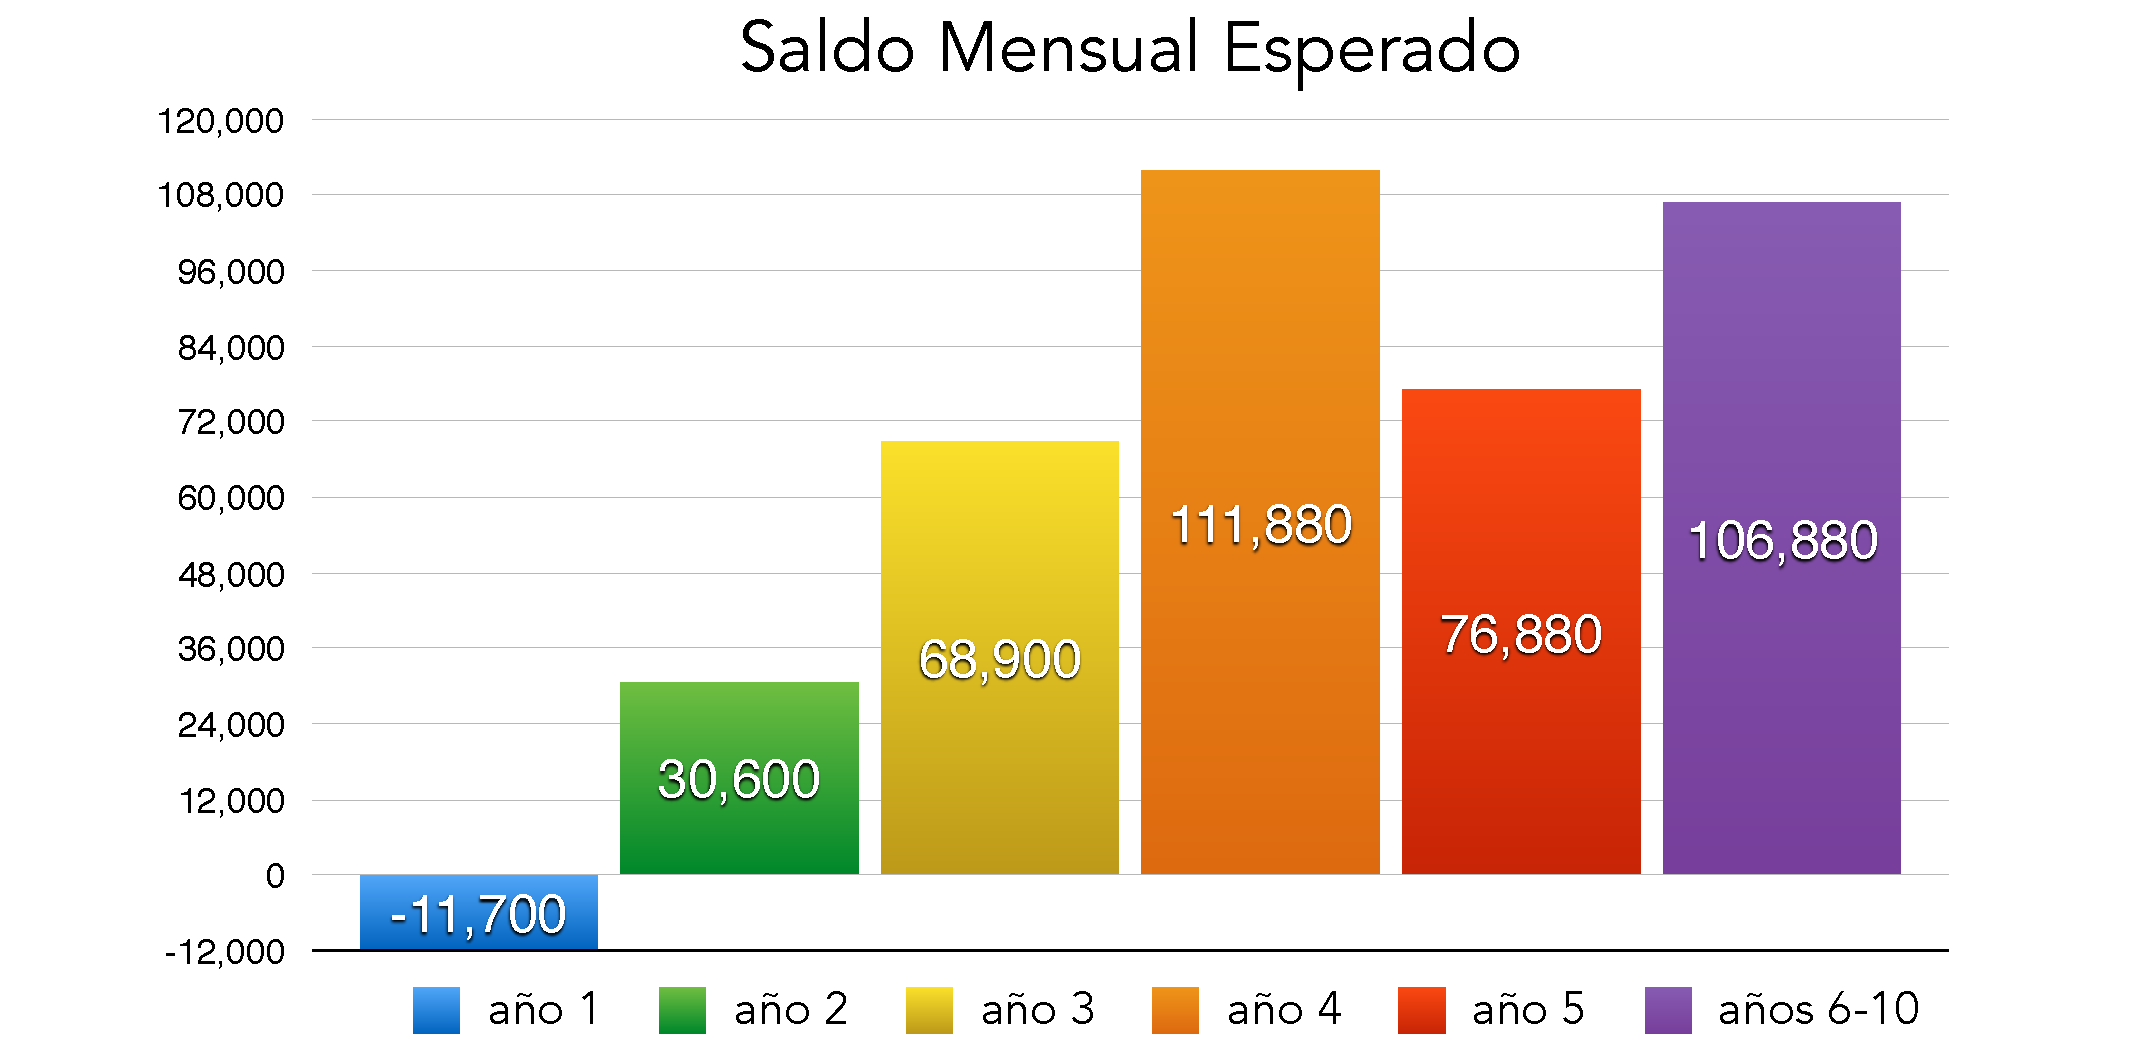
\includegraphics[scale=0.4]{mensual10anos.pdf}
\caption{Saldo mensual proyectado a 10 años.}
\label{mensualProyeccion}
\end{center}
\end{figure}

\section{Inversión y ROI}
\subsection{Escenario Renta}
Se propone una {\bf inversión de un millón de pesos} para rehabilitación del inmueble y compra de mobiliario y adecuaciones estéticas.

\vspace{0.2cm}
{\bf\large \color{red} Siendo así, el Retorno de Inversión se alcanza en 2 años con 2 meses.} como se puede ver en la figura 



\subsection{Escenario Compra}
Se plantea un escenario de {\bf inversión de tres millones y medio de pesos} para la compra de un terreno, construcción y adquisición de inmobiliario.

\vspace{0.2cm}
{\bf\large \color{red} Siendo así, el Retorno de Inversión se alcanza en 7 años con 4 meses.}

\begin{figure}[h]
\begin{center}
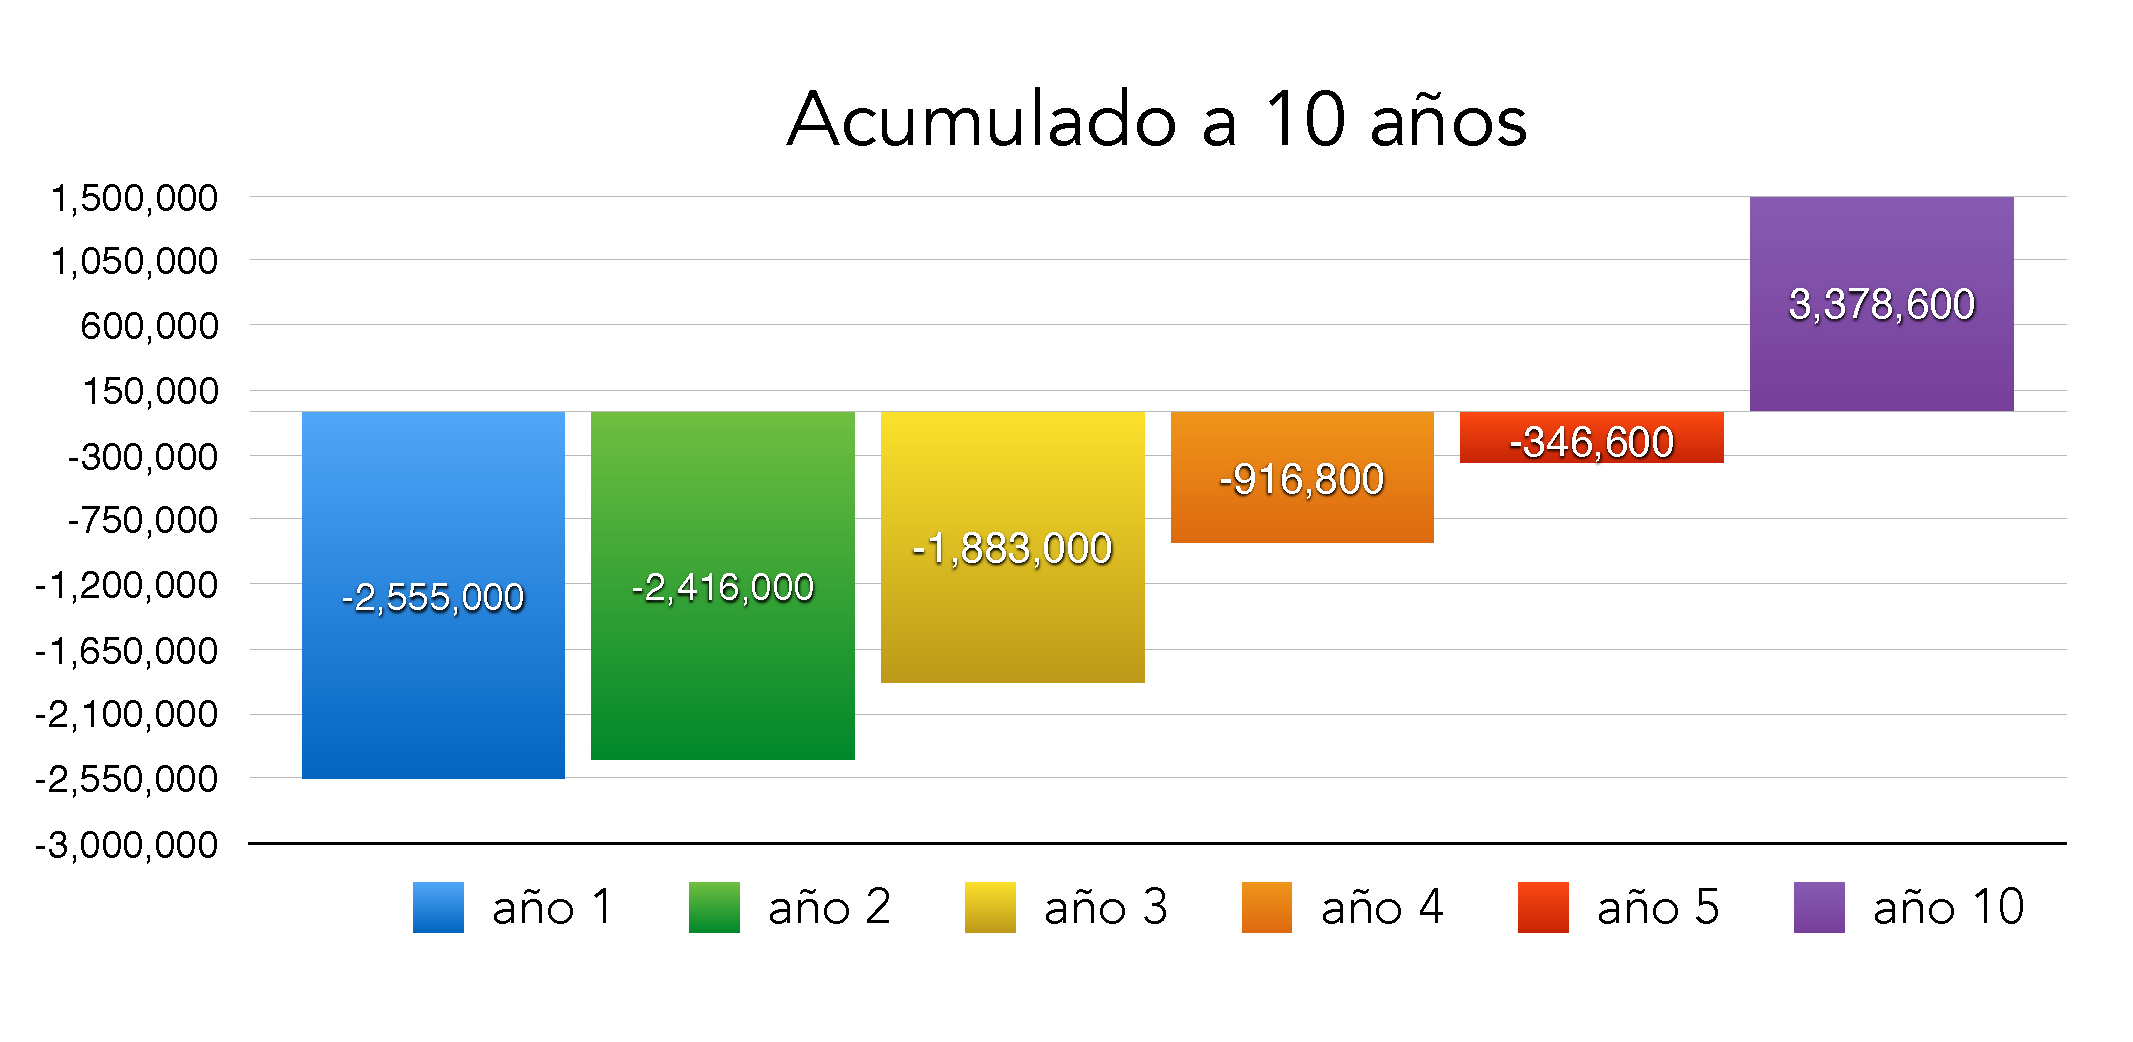
\includegraphics[scale=0.4]{10anos2.pdf}
\caption{Capital neto de Semilla proyectado a 10 años.}
\label{Proyeccion10.1}
\end{center}
\end{figure}

Si la inversión es de {\bf inversión de cuatro millones y medio de pesos} para la compra de un terreno, construcción y adquisición de inmobiliario.

\vspace{0.2cm}
{\bf\large \color{red} Siendo así, el Retorno de Inversión se alcanza en 9 años meses.}

\begin{figure}[h]
\begin{center}
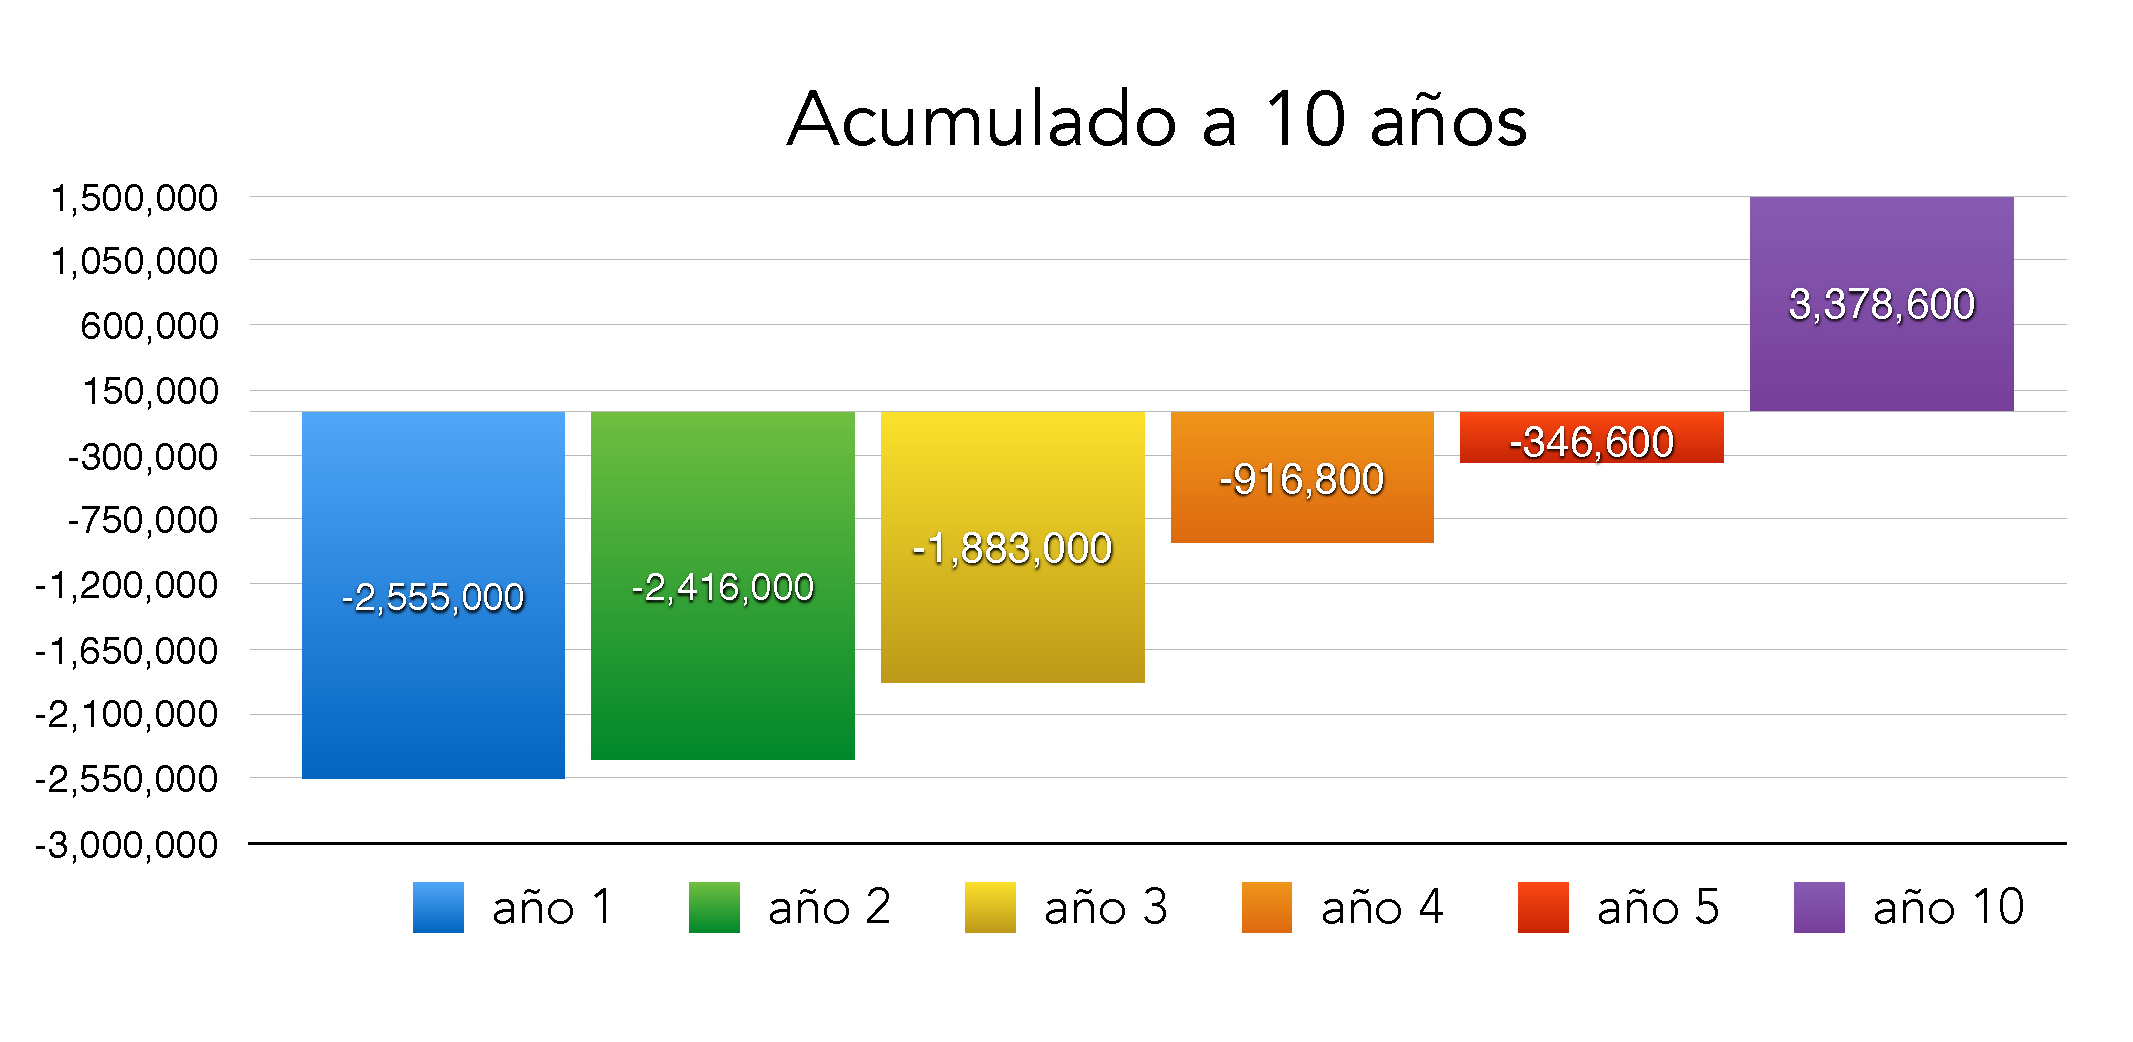
\includegraphics[scale=0.4]{10anos1.pdf}
\caption{Capital neto de Semilla proyectado a 10 años.}
\label{Proyeccion10.1}
\end{center}
\end{figure}

\chapter{Anexos}
	\section{Sobre la forma de publicitar} 
	\subsection{Democracia} Es importante remarcar que la democracia es una palabra pervertida. Para buscar que la gente entienda lo que queremos decir con democracia, debemos ser sutiles y evitar el uso de esa palabra.


\bibliographystyle{IEEEtran}
\bibliography{/Users/e/Documents/bibliography}

\end{document}
